\section{Implementation in C++}
\label{sec:implementation}
%
This section will explain the most important design decisions and technical details on which the implementation of the presented algorithms is based.
While the first priority was clearly to make the code efficient and reduce computation time, another aim was also to create simple and readable code interfaces that make it easy to use and re-use components and extend the existing functionality. \\
%
Even though these two requirements often seem to mutually exclude each other, in this case it was possible to meet both targets.
In fact, it is quite remarkable how similar the C++ implementations of the individual propagators look to their pseudo-algorithms as presented in section \ref{sec:propagators}.
\par\medskip
%
Also, it should be mentioned here that some of the most important bottlenecks of the code were not strictly related to the implementation of the propagators, such as for example the building of the $\bmat{F}$-matrix through numerical quadrature of $\matrixel{\varphi_k}{W}{\varphi_l}$.
In fact, the current implementation of the \proc{build\_matrix} routine for computing the inner product requires to always compute a full $N \times N$ sub-matrix, even if just one single entry is needed, which is a very severe inefficiency if the number of levels $N>1$.
\par\medskip
%
However, the aim of this project was to provide a fast implementation of the propagators by re-using existing functions, therefore possible performance enhancements through changing of the existing code was out of the scope of this project and could be targeted in future work.
Consequently, providing an efficient implementation for time propagation mainly translates into finding an efficient way for calling existing functions with minimal overhead and by making use of compiler optimizations where possible.
\par\medskip
%
First, subsection \ref{subsec:poly} outlines how C++ features were used in order to achieve class inheritance and polymorphism witout any additional runtime cost.
Secondly, in subsection \ref{subsec:callback}, it will be discussed how the \proc{Evolve} method (see algorithm \ref{alg:Evolve}) was implemented in order to provide a minimal working interface to the user while still preserving all the flexibility that may be required for intermediate measurements or other interaction.
Finally, subsection \ref{subsec:intsplit} dives into the technical details of achieving inlined, highly optimized function calls for the \proc{IntSplit} method (see algorithm \ref{alg:intsplit}) that is used intensively in all the presented propagators.
\par\medskip
%
Some details about the code were not found worthy to be mentioned here,
but more information may be found in the Doxygen documentation.
\par\medskip
%
The Hagedorn Propagator was already implemented in C++ as part of another project on the waveblocks library \cite{libwaveblocks}.
Many components of that code were re-used for the present implementation, but they were fundamentally re-organized into a new structure.


\subsection{Static Polymorphism through CRTP and enable\_if}
\label{subsec:poly}
%
In the current software design, all propagators from section \ref{sec:propagators} inherit from a common base class \proc{Propagator}, see the UML diagram \ref{fig:uml}.
The strategy for the implementation was the following:
Provide an efficient and generic implementation of all the building blocks from section \ref{sec:buildingblocks} in a common base class (\proc{Propagator}) and then let the derived class decide which combination of building blocks to use for its own, specific implementation of the propagation methods.
This idea is essentially an application of the Strategy Pattern as introduced by Gamma et al. in \cite{Gamma1995}, one of the most important references for software design patterns.
\par\medskip
%
A popular C++ design pattern for achieving static polymorphism is the \emph{Curiously Recurring Template Pattern}, \emph{CRTP} for short, which is described in more detail in \cite{C_CRTP} and in earlier work on the WaveBlocks project \cite{libwaveblocks}.
\par\medskip
%
While CRTP is an excellent candidate for providing static polymorphism for derived classes, there was also the need for some polymorphism in the Propagator base class itself, since some of the building blocks need to have different implementations based on the dimensionality or homogeneity of the wave packet. 
Providing a partially specialized class for every possible combination of parameters is often tedious and unnecessarily bloats the code.
Therefore, the C++11 \proc{enable\_if} keyword was used.
\proc{enable\_if} allows to define multiple versions of a function and (de)activate them based on a compile-time boolean value.
If the boolean is true, the function is enabled. Otherwise it is omitted.
This handy metafunction from the C++ \proc{type\_traits} header was used in order to conditionally enable functions based on whether the number of levels $N$ was equal or greater to one or to distinguish between functions for homogeneous or inhomogeneous wave functions, which effectively provides a form of compile time polymorphism.
%
\begin{figure}[ht]
	\centering
	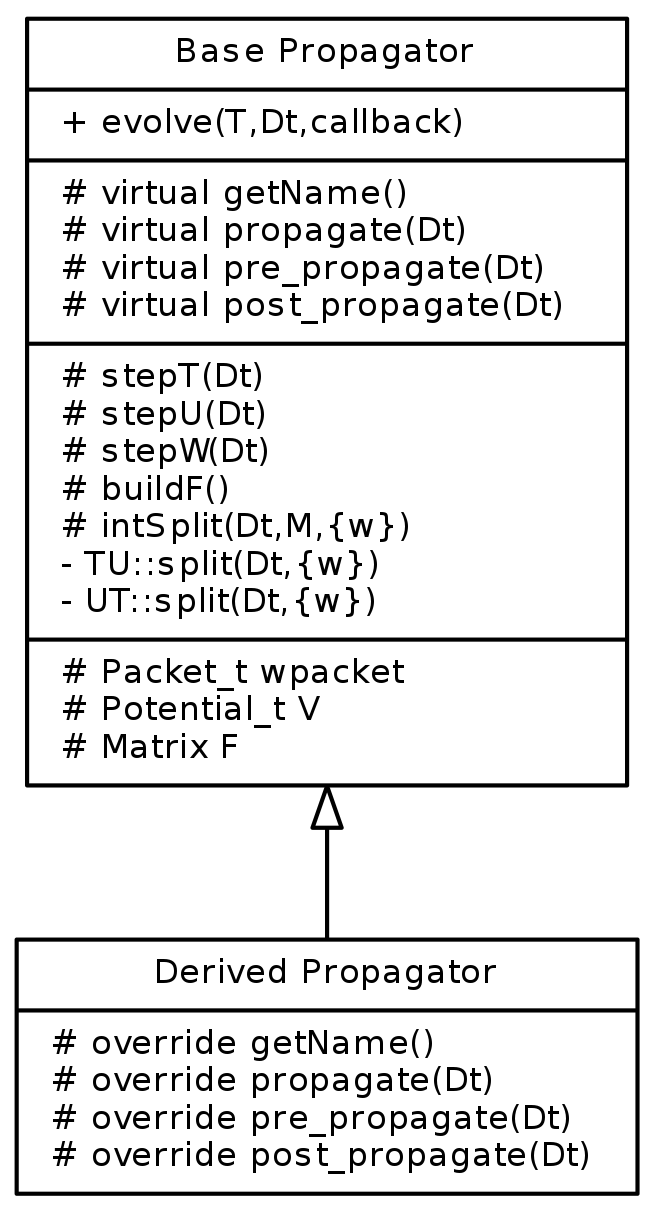
\includegraphics[height=10cm]{figures/uml.png}
	\caption{Simplified UML diagram for the propagator implementation.
		The derived propagator provides implementations for \proc{PrePropagate}, \proc{Propagate} and \proc{PostPropagate} which are called from the public \proc{Evolve} function.
		Some functions and function parameters are omitted for better readability of the graph.}
	\label{fig:uml}
\end{figure}



\subsection{Evolve and callback function}
\label{subsec:callback}
%
The simple \proc{Evolve} method as described in algorithm \ref{alg:Evolve} in the section about propagator building blocks provides a handy wrapper for calling the \proc{PreProcessing}, \proc{Processing} and \proc{PostProcessing} methods in sequence and dividing the propagation time into smaller steps. \\
%
However, one may still want to interact with the wave packet during the simulation, for example for writing the wave packet norm to file every 100 steps, throwing errors when energy conservation is violated or to carry out any other task that requires intermediate simulation results.
In order not to lose any flexibility in this regard, an optional callback-function argument was added to the \proc{Evolve} function.
The callback function is passed as a lambda function taking two arguments, the current simulation time \proc{t} and the index of the current timestep \proc{m}.
If no callback function is passed, it defaults to an empty function.
\par\medskip
%
Furthermore, since the wave packet is passed to the \proc{Propagator} class \emph{by reference}, it is of course available in the callback function as well and does not need to be passed as an argument explicitly (provided that it is captured in the angular brackets \proc{[]} of the lambda function). \\
\emph{Disclaimer} if the value of the wave packet is (intentionally or unintentionally) changed in the callback function, this will of course also affect the further results of the simulation.
Also, care must be taken when measuring energies of packets that are being propagated with propagators such as \emph{Pre764} which apply a pre-processor to the packet before starting the simulation.
In order to get the ``physically correct'' wave packet, the corresponding post-processor needs to be applied before making any meaningful measurement.
\par\medskip
%
The callback function is called once prior to simulation start and then in every time step until termination.
\par\medskip
%
Finally, a few helper functions were introduced in order to facilitate pretty printing of console output and some information about the currently propagated wave packet is printed at the beginning of the \proc{Evolve} function.
These console outputs can (and should) of course be removed for optimal performance, but in most cases it was found that some feedback about the current status of the simulation is highly valuable.


\subsection{IntSplit using alternating templates}
\label{subsec:intsplit}
%
The \proc{IntSplit} function is merely a helper function that alternatingly applies \proc{StepT} and \proc{StepU}.
Steps with the operators $\opT$ and $\opU$ are usually much cheaper than steps with $\opW$ (which requires numerical integration for approximating the inner product $\matrixel{\varphi_k}{W}{\varphi_l}$), but are in many cases found to be one of the main soures of error.
Therefore the idea of sub-dividing the steps into many smaller intervals - an approach introduced in the semiclassical splitting \ref{sub:semiclassical_propagator} - is applied in many other propagators as well.
Consequently, it is desirable to have a generic and efficient implementation available.
\par\medskip
%
The current \proc{IntSplit} algorithm described in \ref{alg:intsplit} takes three arguments:
the size of the time interval to be covered $\Dt$, the number $M_{split}$ of subintervals of size $\dt = \Dt/M_{split}$ in which the initial interval should be divided, and a pair of coefficient lists $\{ w_T, w_U \}$ denoting the weights with which the single steps of size $\dt$ should be scaled.
In the simplest case, the lists $w_T$ and $w_U$ are both only of length one (Lie-Trotter), but higher order splitting strategies can have much larger coefficient sets.
In general, it must hold that $\text{length}(w_T) = \text{length}(w_U)$ (for TU..TU schemes) or $\text{length}(w_T) = \text{length}(w_U)$ (for TU..UT schemes).
\par\medskip
%
The obvious implementation of using a dynamic container (like a C++ vector) for the coefficients and a simple \emph{for loop} over all its entries brings a two (minimal) drawbacks: First, the overhead of the loop itself and second, the fact that the number of coefficients is not known at compile time and thus no optimizations can be done.
Given that the functions \proc{StepT} and \proc{StepU} themselves are very cheap (just simple updates of parameters $\bvec{\Pi}$ and $S$), it is preferable to remove any kind of additional cost, even if only marginal.
\par\medskip
%
By making use of C++ arrays and templates, one can remove the issues mentioned above. \\
%
Firstly, by replacing C++ vectors (dynamically allocated) through C++ arrays (statically allocated), the container size is known at compile time.
For convenience, a new struct \proc{SplitCoefs} was introduced that holds a pair of such arrays.
Secondly, and with the information about container size readily available at compile time, one can then implement two sets of templates \proc{TU} and \proc{UT} that execute a step with operator $\opT$ or $\opU$ respectively and then mutually invoke each other, until both arrays of coefficients are used up.
As a termination condition, when all coefficients have been used, a partially specialized instance of the templates will be called and interrupt the mutual invocation. \\
%
One technical subtlety of this approach is, that the C++ language does not allow partially specialized function templates. This can, however, be overcome quite easily by declaring \proc{TU} and \proc{UT} as classes with a static function.
In contrast to function templates, class templates can be partially specialized.
By using static member functions, the actual class objects do not need to be created and all the function calls will be resolved at compile time.
\footnote{One limitation is the maximal template recursion depth. The default value on gcc compiler is 900 and can be increased if required. Typical template nesting depths for coefficient pairs should lie significantly below 100.}
All templates, no loops, and the resulting sequential code can then be further optimized by the compiler.
\par\medskip
%
Some minimal code snippets explaining the working principle of \proc{IntSplit} are shown in figure~\ref{fig:intsplit}
%
In order to prevent the inappropriate use of the \proc{IntSplit} function through incompatible coefficient lists $w_T$ and $w_U$, their sizes are checked in the code at compile time via static assertions.
\par\medskip
%
The fact that $\opW$ is significantly more costly to compute than its counterparts $\opT$ and $\opU$ also justifies the approach of using templates that are hard-coded to call functions \proc{StepT} and \proc{StepU}, as these are the only logical candidates for \proc{IntSplit}.

\begin{figure}[ht]
	\begin{minipage}[c]{\textwidth}
		\begin{minipage}[l][10cm][t]{.4\textwidth}
			\begin{minipage}[t]{\textwidth}
\begin{lstlisting}
// Specialized Template
// N_T == S_T
// N_U == S_U
template <int S_T,int S_U>
struct TU<S_T,S_U,S_T,S_U> {
	static void split(
	   array<float,S_T>& w_T,
	   array<float,S_U>& w_U,
		 float dt)
	{ /* terminate */ }
};
\end{lstlisting}
			\end{minipage} \\
			\vspace{5mm}
			\begin{minipage}[t]{\textwidth}
\begin{lstlisting}
template <int N_T,int N_U,
           int S_T,int S_U>
struct TU {
	static void split(
	  array<float,S_T>& w_T,
	  array<float,S_U>& w_U,
		float dt)
		/* T */
		stepT(w_T(N_T)*dt);
		/* UT... */
		UT<N_U,N_T+1,S_U,S_T>
		   ::split(w_U,w_T,dt);
	}
};
\end{lstlisting}
			\end{minipage}
	\end{minipage}
		\begin{minipage}[l][10cm][t]{.18\textwidth}
			\vspace{25mm}
		\resizebox{\textwidth}{!}{
\begin{tikzpicture}[->,>=stealth',auto,node distance=3cm,
  thick,main node/.style={circle,draw,font=\sffamily\Large\bfseries}]
					\node (TU) at (0,0) {};
					\node (UT) at (2,0) {};
					\node (TUexit) at (0,2) {};
					\node (UTexit) at (2,2) {};
					\node (TUend) at (0,4) {};
					\node (UTend) at (2,4) {};
				\path[every node/.style={font=\sffamily\small}]
					(TU) edge[bend right] node {} (UT)
					(UT) edge[bend right] node {} (TU)
					(TUexit) edge node {} (UTend)
					(UTexit) edge node {} (TUend);
\end{tikzpicture}
			}
		\end{minipage}
	\begin{minipage}[r][10cm][t]{.4\textwidth}
			\begin{minipage}[t]{\textwidth}
\begin{lstlisting}
// Specialized Template
// N_U == S_U
// N_T == S_T
template <int S_U,int S_T>
struct UT<S_U,S_T,S_U,S_T> {
	static void split(
	   array<float,S_U>& w_U,
	   array<float,S_T>& w_T,
		 float dt)
	{ /* terminate */ }
};
\end{lstlisting}
			\end{minipage} \\
			\vspace{5mm}
			\begin{minipage}[t]{\textwidth}
\begin{lstlisting}
template <int N_U,int N_T,
           int S_U,int S_T>
struct UT {
	static void split(
	  array<float,S_U>& w_U,
	  array<float,S_T>& w_T,
		float dt)
		/* U */
		stepU(w_U(N_U)*dt);
		/* TU... */
		TU<N_T,N_U+1,S_T,S_U>
		   ::split(w_T,w_U,dt);
	}
};
\end{lstlisting}
			\end{minipage}
	\end{minipage}
	\end{minipage}
	\caption{Simplified C++ snippets for outlining the template invocation sequence in the \proc{IntSplit} function. The template parameters \proc{S\_T} and \proc{S\_U} denote the total size of the coefficient arrays \proc{w\_T} and \proc{w\_U} while the \proc{N\_T} and \proc{N\_U} are the indices of the current coefficient to be applied. The \proc{TU::split} and \proc{UT::split} methods first apply their own step and then invoke each other by gradually incrementing the incices \proc{N\_T} and \proc{N\_U}. \\
	When the conditions \proc{N\_T == S\_T} and \proc{N\_U == S\_U} are satisfied, the partially specialized templates become active and the recursion is terminated.}
	\label{fig:intsplit}
\end{figure}
